% Template for Cogsci submission with R Markdown

% Stuff changed from original Markdown PLOS Template
\documentclass[10pt, letterpaper]{article}

\usepackage{cogsci}


\title{Idiosyncratic but not opaque: Linguistic conventions formed in
reference games are interpretable by naïve humans and vision--language
models}

\usepackage{booktabs}
\raggedbottom

\author{anon}


\begin{document}

\maketitle

\begin{abstract}
When are in-group linguistic conventions opaque to non-group members
(teen slang like ``rizz'') or generally interpretable (regionalisms like
``roundabout'')? The formation of linguistic conventions is often
studied in iterated reference games, where over repeated reference to
the same targets, a describer--matcher pair establishes partner-specific
shorthand names for targets. To what extent does the partner-specificity
of these linguistic conventions cause them to be opaque to outsiders? We
use computational models and experiments with naïve matchers to assess
the opacity of descriptions from iterated reference games. Both human
matchers and the computational model perform well above chance,
suggesting that conventions are not fully arbitrary or opaque, but
reflect aspects of shared semantic associations.

\textbf{Keywords:}
reference games; convention formation; computational modeling; opacity;
pragmatics
\end{abstract}

\section{Introduction}\label{introduction}

When a teen says about someone that ``he's got rizz,'' what does this
mean? The idea that teen slang is arbitrary and opaque to outsiders
(i.e., older generations) is enough of a cultural touchstone that late
night comedy shows have segments about it. Teens are far from the only
ones to have in-group naming conventions; many communities form stable
linguistic conventions including professional jargon, regionalisms, and
of course slang.

The formation of linguistic conventions between individuals is often
studied experimentally in iterated reference games. In these games, a
describer tells their partner how to sort or match a series of abstract
images (e.g., Clark \& Wilkes-Gibbs, 1986; Hawkins et al., 2020). Over
repeated rounds of referring to the same targets, pairs develop
conventionalized nicknames for the target images. These nicknames are
often partner-specific, in that different pairs develop different
nicknames for the same targets. When describing the targets to a new
person, describers return to more elaborated descriptions, indicating an
expectation that prior conventions are not appropriate descriptions to
use for new matchers (Hawkins, Liu, et al., 2021; Wilkes-Gibbs \& Clark,
1992; Yoon \& Brown-Schmidt, 2018).

For one-shot reference games, the choice of referring expression can be
described as a process of recursive inference, in which speakers reason
about how listeners will interpret their utterance and vice versa. This
process is described in Bayesian pragmatics models such as the Rational
Speech Acts model (RSA) (Frank \& Goodman, 2012; Goodman \& Frank,
2016). The Continual Hierarchical Adaptation through Inference model
(CHAI) builds on RSA by adding rules for how agents update their belief
distributions after each interaction, to account for the dynamics of
repeated interaction in iterated reference games (Hawkins, Franke, et
al., 2021). A key factor permitting variation in referring expressions
is lexical uncertainty; RSA models incorporating lexical uncertainty
(Bergen et al., 2016; Potts et al., 2016) treat listeners as Bayesian
agents who jointly infer the meaning of a speaker's utterance and their
model of the speaker's lexicon. Models incorporating lexical uncertainty
have been used to model children's word learning (Bohn et al., 2022) as
well as person- and group-level differences (Hawkins, Franke, et al.,
2021; Schuster \& Degen, 2020). Usually the scope of person-to-person
variation in lexica is constrained, so it is more akin to learning a
hierarchical set of tweaks to a lexicon so some words have slightly
different extensions for different speakers and different circumstances,
rather than learning completely arbitrary meanings for each person
(Hawkins, Franke, et al., 2021; Schuster \& Degen, 2020; but see Misyak
et al., 2016).

Conventions in iterated reference games are formed between people
without a salient shared group identity prior to the interaction, but
people do not use the conventions with new partners. How opaque are the
temporary linguistic conventions created in reference games: are they
opaque like ``rizz'' or interpretable like ``roundabout''? From a
theoretical perspective, measuring this opacity can help inform the
development of models like CHAI that aim to account for lexical change
in conversation. We attempt to answer this question here.

One way to measure the opacity of a referring expression is to look at
the semantic distance between the signifier and the referent.
Expressions that are more transparent are those where signifiers and
referents are semantically close, such that anyone with the same general
lexicon can identify the appropriate referent given the signifier. In
contrast, expressions that are opaque have signifiers and referents that
are semantically distant in the lexicon, such that the relations are
arbitrary and inaccessible without additional clues such as the
partner-specific conversation history.

One option for measuring the transparency of referring expressions is to
use vision--language models to operationalize a shared semantic space
for both language and images. Computational methods have enabled the
embedding of various stimuli (including images and text) into
high-dimensional feature spaces; these embeddings have properties which
suggest that they are reasonable approximations of humans' semantic
spaces, including similarity in representational geometries (e.g., Grand
et al., 2022; Muttenthaler \& Hebart, 2021). Indeed, embeddings from
neural network models have been used as a form of semantics in a range
of reference game scenarios (e.g., Gul \& Artzi, 2024; Ji et al., 2022;
Kang et al., 2020; Le et al., 2022; Ohmer et al., 2022). In particular,
such embeddings can be treated as the default context- and
speaker-independent lexicon, since they are not updated to account for
convention formation within an iterated reference game.

A second option for measuring the transparency of referring expressions
is to measure how often naïve humans, who were not part of the group who
formed the convention, can correctly associate the target referent with
the referring expression. Prior work with naïve matchers has been
limited and has focused on the role of conversational history. In this
work, naïve matchers tend to do better the more their observation
history resembles that of the original conversation---when hearing
descriptions in order instead of in reverse order (Murfitt \&
McAllister, 2001), when listening to the entire game instead of starting
in the third round (Schober \& Clark, 1989), and when seeing yoked
trials from a single game rather than trials sampled across 10 games
(Hawkins et al., 2023). In these studies, naïve matchers had worse
accuracy than in-game matchers, but their performance was still far
above chance, suggesting that the convention--target relationship is not
purely arbitrary. In fact, even when pairs of participants try to
obfuscate their meaning, overhearers can still do quite well at
identifying the target referents (Clark \& Schaefer, 1987). Nonetheless,
receiving more context from an interaction---and in particular having
that context be in order---is beneficial to matchers.

In the current work, we measure the opacity of the referring expressions
created in iterated reference games. We use conversations from Boyce et
al. (2024), who created a large corpus of iterated reference games that
were played online using a chatbox for communication. This corpus is
made up of 6-round iterated reference games using the same 12 target
images. Games varied in how large the describer--matcher groups were
(2--6 participants) and how ``thick'' the communication channels were
(for example, if matchers could send back messages or just emoji). The
varied conditions within a consistent framework allowed us to test how
the opacity of referring expressions varies depending on the conditions
the referring expressions came from.

We use both human experiments and models to assess when and why
expressions are opaque or understandable to outside observers. We first
present a computational approach using a vision--language model to
measure the semantic similarities between referring expressions and
their targets, and we validate our model against naïve human matchers
(Experiment 1). We then use both naïve human matchers and the model to
compare the opacity of referring expressions across different game
conditions and time points (Experiment 2). Finally, we address the role
of conversation history by comparing naïve matcher performance on game
transcripts presented in order versus out of order (Experiment 3).

\begin{CodeChunk}
\begin{figure}[t!]

{\centering 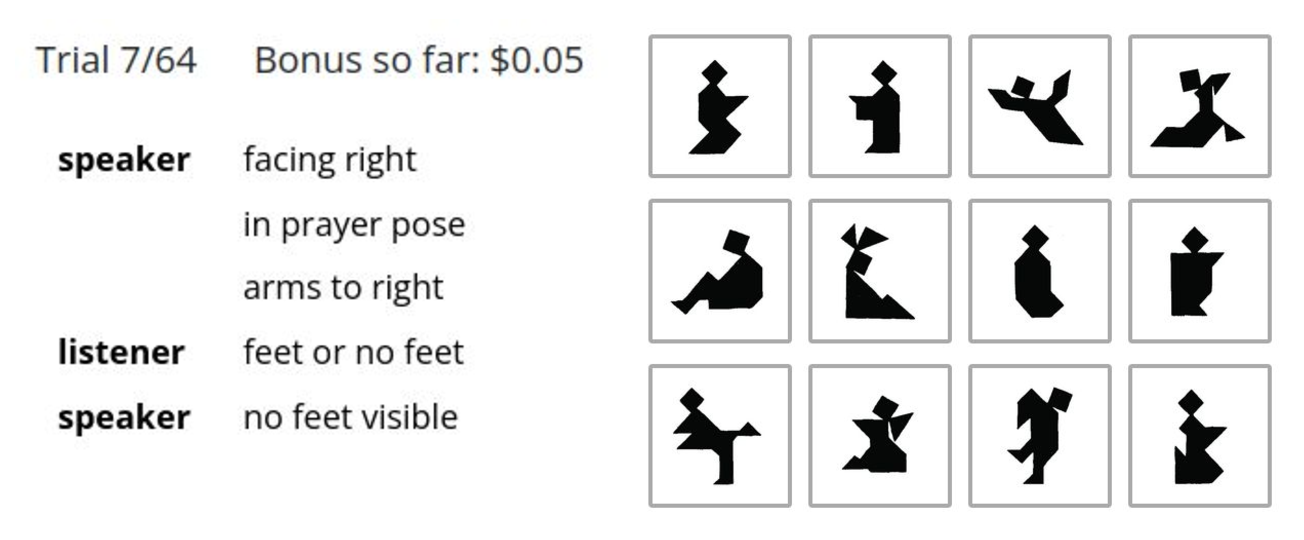
\includegraphics[width=1\linewidth]{matcher-diagram} 

}

\caption[Experimental setup]{Experimental setup. Naïve matchers read transcripts from trials in reference games from Boyce et al. (2024) and selected which image they thought was being described. Matchers recieved bonus payments for correct selections. \label{game}}\label{fig:interface}
\end{figure}
\end{CodeChunk}

\section{Task setup}\label{task-setup}

\subsection{Materials}\label{materials}

We drew our referring expressions from Boyce et al. (2024), excluding
utterances that were marked as not containing referential content. For
our naïve matcher experiments, we sampled different subsets of this
corpus. Within the subsets, we excluded transcripts that contained swear
words or crude or sexual language. For the computational model, we used
the entire corpus, and pre-processed the text by concatenating all the
referential messages sent by the describer for a given trial.

\subsection{Experimental procedure}\label{experimental-procedure}

We recruited English-speaking participants from Prolific. On each trial,
participants saw the full transcript from that trial, containing all the
chat messages marked by whether they were from the speaker or a
listener. Participants selected the image they thought was the target
from the tableau of 12 (Figure \ref{game}). Participants received
feedback on whether they were right or wrong on each trial. Except when
the specific viewing order was part of the experimental manipulation, we
randomized the order of trials, subject to the constraint that the same
target could not repeat on adjacent trials. The task was implemented in
jsPsych (Leeuw et al., 2023). We paid participants \$10 an hour plus a
bonus of 5 cents per correct response. All our experimental code is at
\href{https://osf.io/bfk8y/?view_only=165b81c5d69446f18e1bfd23e3d9cb5f}{this
anonymized repo}.

\subsection{Computational models}\label{computational-models}

We used the Contrastive Language-Image Pretraining model (CLIP;
\texttt{clip-vit-large-patch14}) as a comprehender model for our domain
(Radford et al., 2021). CLIP is a vision-language model that uses a text
transformer and a vision transformer to embed text and images into the
same space, trained to maximize the similarity between representations
of images and their English captions. It is a natural choice for
reference games, as the model is trained to estimate the correspondence
between images and phrases in natural language. We ran CLIP for the
concatenated describer utterances and all 12 tangram shapes. For each
utterance, we computed probabilities for each tangram shape using logit
scores from CLIP. The simplest way to do this is simply taking the
softmax of the logits. However, tangram shapes are outside of the
training distribution for the model, perhaps explaining why it favored
some images over others regardless of the content of the text.

\begin{table}
\caption{Cross-validated accuracies for classifiers. Standard deviations in accuracy across the 10 folds are shown in parentheses. Best performance within each model class is underlined, and best overall performance is bolded.}
\label{tab:classifier_comparison}
\centering
\small
  \begin{tabular}{p{1em}lr}
    \toprule
    \multicolumn{2}{l}{Classifier} & Accuracy \\ 
    \midrule
        \multicolumn{2}{l}{Random baseline} & \smash{0.08} \\
    \multicolumn{2}{l}{CLIP without readout} & \smash{0.31} \\
    \multicolumn{2}{l}{Logistic regression} & \\
    & No penalty & \underline{\smash{0.50 (0.01)}} \\ 
    & \vspace{1mm}L2 penalty & 0.50  (0.01) \\ 
    \multicolumn{2}{l}{Random forest} & \\
    & 10 estimators & 0.46 (0.02) \\
    & 50 estimators  & 0.51 (0.02)\\ 
    & 100 estimators & 0.52 (0.02) \\ 
    & \vspace{1mm}500 estimators & \underline{\smash{0.52 (0.02)}} \\ 
    \multicolumn{2}{l}{Gradient-boosted tree} & \\
    & 10 estimators & 0.48 (0.02) \\ 
    & \vspace{1mm}100 estimators & \underline{\smash{0.51 (0.02)}} \\ 
    \multicolumn{2}{l}{Multi-layer perceptron} & \\
    & 1 $\times$ 32-dim hidden layer & 0.50 (0.01) \\ 
    & 1 $\times$ 100-dim hidden layer  & 0.52 (0.01) \\ 
    & 1 $\times$ 512-dim hidden layer & 0.53 (0.02) \\ 
    & 1 $\times$ 1028-dim hidden layer & 0.53 (0.02) \\ 
    & 2 $\times$ 32-dim hidden layers  & 0.51 (0.02) \\ 
    & 2 $\times$ 100-dim hidden layers & \underline{\smash{\textbf{0.55 (0.02)}}} \\ 
    \bottomrule
    \end{tabular}
\end{table}

To improve the performance of base CLIP, we trained a set of readout
models to assign probabilities to images using CLIP's logits as
features. Models were trained to maximize task performance (i.e., to
assign high probability to the target tangram given the concatenated
describer utterance). We compared four types of models: random forest,
logistic regression, multi-layer perceptron (MLP), and gradient-boosted
tree. Classifiers were implemented in the \texttt{scikit-learn} and
\texttt{XGBoost} libraries (Chen \& Guestrin, 2016; Pedregosa et al.,
2011). Each readout model was evaluated using 10-fold cross-validation,
where the model was trained on 90\% of the data and evaluated on the
remaining 10\%. Table \ref{tab:classifier_comparison} shows the
cross-validated accuracy of different readout models, as well as the
performance of CLIP with no readout. The MLP with two hidden layers of
size 100 performed the best on held-out data; in subsequent analyses, we
use the MLP trained on all the data.

\section{Experiment 1}\label{experiment-1}

\begin{CodeChunk}
\begin{figure}[t]

{\centering 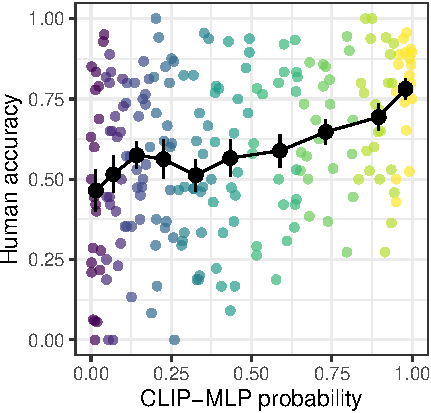
\includegraphics[width=0.7\linewidth]{figs/fig-calibration-1} 

}

\caption[Correlation between human accuracy and CLIP-MLP probability of target in Experiment 1]{Correlation between human accuracy and CLIP-MLP probability of target in Experiment 1.  Small points are individual descriptions, colored by decile of CLIP-MLP probability, large points and error bars are the bootstrapped mean and 95\% CI across descriptions for each decile. \label{calibration}}\label{fig:fig-calibration}
\end{figure}
\end{CodeChunk}

Our CLIP-MLP computational model was optimized for task accuracy. To
validate whether this objective also results in human-like response
patterns, we conducted a calibration experiment to determine if
model-assigned target probabilities were aligned with the probabilities
that naïve human matchers would choose particular target images across a
range of utterance-target pairs.

\subsection{Methods}\label{methods}

We first obtained target probabilities from our CLIP-MLP model for all
utterances from Boyce et al. (2024). We then used stratified sampling to
select 217 trials by dividing model-predicted probabilities into deciles
and choosing approximately 22 utterances per decile, spanning the 12
different possible target images. We recruited 61 participants who each
saw 64 trials randomly sampled from the 217 tested trials. On average,
each trial was seen by 18 participants. This experiment was
pre-registered at
\href{https://osf.io/6pv5e/?view_only=0bc61ddeda83493c844ca554f463ba85}{this
anonymized link}.

\subsection{Results and discussion}\label{results-and-discussion}

We obtained human accuracies on each trial by dividing the number of
participants who selected the target by the total number of participants
who saw the trial (Figure \ref{fig:fig-calibration}). There was a modest
but significant positive correlation between model-predicted
probabilities and human accuracies (\(r\) = 0.33 {[}0.21, 0.45{]}). This
result suggests that model predictions were calibrated to human response
patterns, albeit not perfectly. Nonetheless, the observed positive
correlation suggests that our computational model carries some signal
about human accuracies, validating its use in subsequent experiments as
a computational comparison.

\begin{CodeChunk}
\begin{figure}[t]

{\centering 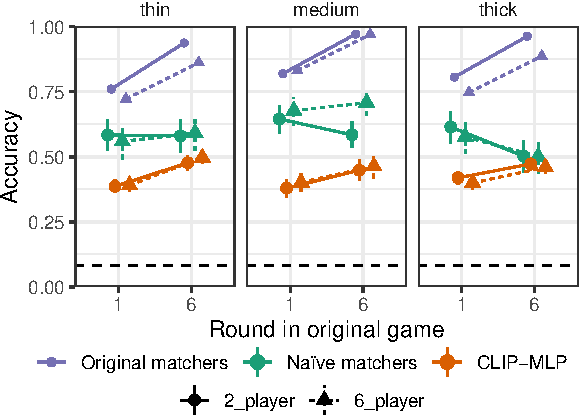
\includegraphics[width=0.9\linewidth]{figs/fig-condition-1} 

}

\caption[Accuracies for naïve human matchers and the CLIP-MLP model for Experiments 2a and 2b, grouped by the source of the referential description]{Accuracies for naïve human matchers and the CLIP-MLP model for Experiments 2a and 2b, grouped by the source of the referential description. Facets are the communication thickness of the original game and x-axis is when in the game the transcript came from. Point estimates and 95\% CrI are predictions from the fixed effects of logistic and beta regressions. Bootstrapped mean accuracy from the original matchers is included as a ceiling, and random chance as a baseline. \label{expt2-condition}}\label{fig:fig-condition}
\end{figure}
\end{CodeChunk}

\begin{CodeChunk}
\begin{figure}[t]

{\centering 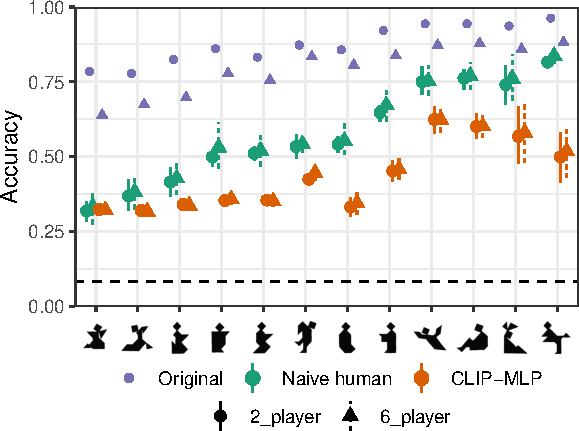
\includegraphics[width=0.9\linewidth]{figs/fig-2-1} 

}

\caption[Accuracies for naïve human matchers and the CLIP-MLP model for Experiments 2a and 2b, split out by target image]{Accuracies for naïve human matchers and the CLIP-MLP model for Experiments 2a and 2b, split out by target image. Point estimates and 95\% CI are predictions from the fixed effects and by-tangram random effects of logistic and beta regressions, bootstrapped across conditions. Bootstrapped mean accuracy from the original matchers is included as a ceiling, and random chance as a baseline. \label{expt2-tangram}}\label{fig:fig-2}
\end{figure}
\end{CodeChunk}

\section{Experiment 2}\label{experiment-2}

As a starting point for examining the opacity of referring expressions,
we focused on referring expressions from the first and last rounds of
reference games. Based on the idea that conventions form across repeated
communication, later-round utterances should be more opaque. To test
this hypothesis, we ran a recognition experiment including descriptions
from games of different sizes and communication thicknesses. Based on
the patterns of cross-game similarity in Boyce et al. (2024), we
expected that smaller and thicker games, whose descriptions diverged
fastest, would have more idiosyncratic and opaque conventions than
larger groups with thinner communication channels.

\subsection{Methods}\label{methods-1}

\subsubsection{Experiment 2a}\label{experiment-2a}

To establish a baseline of how well naïve matchers could understand
descriptions without context, we ran a 2 \(\times\) 2 within-subjects
experiment, drawing target transcripts from 2- and 6-player games from
Experiment 1 of Boyce et al. (2024) and from the first and last blocks
of these games. These games had medium-thick communication channels,
where matchers could send text messages to the chat, the describer role
rotated each round, and matchers received limited feedback. We recruited
60 participants who each saw 60 trials (15 in each of the 4 conditions).
Overall, participants saw 774 transcripts from 40 games. This experiment
was pre-registered at
\href{https://osf.io/k45dr/?view_only=1f4bbadb8e6b4b5f8d04cf04392967dd}{this
anonymized link}.

\subsubsection{Experiment 2b}\label{experiment-2b}

After observing limited condition differences in Experiment 2a, we ran a
follow-up experiment on descriptions from Experiment 3 of Boyce et al.
(2024), where the communication channel thicknesses were more extreme.
Here, we used a 2 \(\times\) 2 \(\times\) 2 within-subjects design,
drawing our transcripts from the first and last rounds of thick and
thin, 2- and 6- person games. In the ``thick'' condition, matchers could
send text messages to the chat, one person was the describer for the
whole game, and matchers received feedback on everyone's selections. In
contrast, in the ``thin'' condition, matchers could only communicate by
sending 4 emoji, the describer role rotated, and matchers recieved
limited feedback. As the emoji did not have referential content, we did
not include them in the transcripts shown to naïve matchers. For
experiment 2b, we recruited 60 participants who each saw 64 trials (8 in
each of the 8 conditions). Overall, participants saw 2392 transcripts
from 163 games. This experiment was pre-registered at
\href{https://osf.io/rdp5k/?view_only=87452ac1a7894f98b51b5642346e9e3d}{this
anonymized link}.

\subsection{Results}\label{results}

\subsubsection{Experiment 2a}\label{experiment-2a-1}

For Experiment 2a, we ran a Bayesian mixed-effects logistic model of
naïve matcher accuracy in \texttt{brms} (Bürkner, 2018).\footnote{correct
  \({\sim}\) group\_size \({\times}\) round~\({+}\) trial\_order~\({+}\)
  (group\_size \({\times}\) round\textbar correct\_tangram)~\({+}\)
  (group\_size \({\times}\) round~\({+}\) trial\_order\textbar workerid)}
Overall, naïve matchers were right 62\% of the time, far above the 1/12
= 8.3\% expected by random chance (OR = 1.93 {[}1.05, 3.62{]}). There
were no large effects of condition (Figure \ref{expt2-condition} middle
panel). Participants tended to be less accurate at descriptions from the
last round (OR of last round = 0.77 {[}0.53, 1.10{]}). There was no
clear effect of original group size (OR of 6-player game = 1.15 {[}0.89,
1.47{]}), but there was an interaction between round and group size (OR
= 1.49 {[}1.06, 2.10{]}). Later transcripts from larger games were
easier to understand, but earlier transcripts from smaller games were
easier to understand. Much of the variation in accuracy was driven by
the target image, which accounted for more variation than participant
differences (standard deviation of image distribution = 0.98 {[}0.63,
1.51{]}; SD of participant distribution = 0.64 {[}0.42, 0.88{]}). Some
images were much easier to identify as the target than others (Figure
\ref{expt2-tangram}).

\subsubsection{Experiment 2b}\label{experiment-2b-1}

For Experiment 2b, we ran a similar Bayesian mixed-effects logistic
model.\footnote{correct \({\sim}\) group\_size \({\times}\) thickness
  \({\times}\) round~\({+}\) trial\_order~\({+}\) (group\_size
  \({\times}\) thickness \({\times}\)
  round\textbar correct\_tangram)~\({+}\) (group\_size \({\times}\)
  thickness \({\times}\) round~\({+}\) trial\_order\textbar workerid)}
Naïve matchers were above chance (OR = 1.81 {[}1.06, 3.08{]}, Figure
\ref{expt2-condition}). As in Experiment 2a, there were not substantial
effects of condition. Last-round descriptions had slightly lower
accuracy (OR of last round = 0.64 {[}0.47, 0.85{]}), but there was an
interaction with thickness, where for thin games, last round
descriptions were less opaque (OR = 1.55 {[}1.02, 2.33{]}). Again there
was strong variation based on target image (0.81 {[}0.51, 1.28{]}),
which exceeded by-participant variation (0.62 {[}0.43, 0.83{]}).

\subsubsection{Additional predictors}\label{additional-predictors}

We considered the accuracy of the in-game matchers from Boyce et al.
(2024) and the length of the description as post-hoc predictors. In both
experiments, in-game accuracy was predictive of naïve matcher accuracy
(Expt 2a OR = 3.33 {[}2.45, 4.53{]}, Expt 2b OR = 2.39 {[}1.88,
3.03{]}). The log number of words in the description was not predictive
in Experiment 2a (OR = 1.05 {[}0.94, 1.17{]}), but longer descriptions
were slightly beneficial in Experiment 2b (OR = 1.10 {[}1.01, 1.20{]}).

The pattern of which conditions became more opaque in later rounds
resembled the pattern of which conditions produced descriptions that
diverged the most in semantic space in Boyce et al. (2024). As a
post-hoc test of whether opacity might be related to semantic
divergence, we used the mean semantic similarity between an utterance
and other utterances in the same condition as an additional predictor of
accuracy.\footnote{Semantic similarity was operationalized as cosine
  similarity between S-BERT embeddings (Reimers \& Gurevych, 2019), the
  measure of semantic distance used in Boyce et al. (2024).} Similarity
to other utterances was strongly predictive of increased accuracy in
both experiments (Expt 2a: OR = 12.49 {[}4.70, 33.64{]}, Expt 2b: OR =
14.75 {[}5.93, 36.87{]}) and was more predictive for the last round
descriptions (Expt 2a: OR = 3.49 {[}1.09, 10.92{]}, Expt 2b: OR = 4.78
{[}1.61, 14.25{]}). While exploratory, this analysis suggests that
referring expressions that are further from shared semantic priors
(i.e., more idiosyncratic) are harder for naïve matchers to understand.

\subsection{Model results}\label{model-results}

As a computational comparison, we used the probability the CLIP-MLP
model assigned to the correct target as our dependent measure and fit a
Bayesian mixed-effects beta regression on the descriptions from
Experiment 2.\footnote{correct \({\sim}\) group\_size \({\times}\)
  thickness \({\times}\) round~\({+}\) (group\_size \({\times}\)
  thickness \({\times}\) round\textbar correct\_tangram)} The CLIP-MLP
model was far above chance, but had lower accuracy than the human
participants (OR = 0.60 {[}0.45, 0.82{]}). The strongest predictor of
accuracy was later round (OR = 1.32 {[}0.94, 1.83{]}), but even this was
uncertain. There was substantial by-target image variation (SD = 0.46
{[}0.27, 0.76{]}).

In additional models, we checked the effect of in-game matcher accuracy,
length of the description, and semantic divergence. CLIP-MLP had higher
accuracy when in-game matcher accuracy was higher (OR = 1.52 {[}1.35,
1.71{]}), and when descriptions were shorter (OR for log words = 0.85
{[}0.82, 0.90{]}). The model may perform poorly on long descriptions
because they are further from the model's training distribution of image
captions. A description's semantic similarity to other descriptions was
predictive of higher accuracy (OR = 11.85 {[}6.51, 21.06{]}), especially
for last round utterances (OR = 3.46 {[}1.65, 7.36{]}), in line with the
human results.

\subsection{Discussion}\label{discussion}

Overall, naïve human matchers were fairly accurate overall, but less
accurate than matchers in the original game, consistent with prior work.
The computational model was less accurate, but still far above chance.
The largest source of variability in accuracy was from target images,
and whether earlier or later utterances were more opaque varied by game
condition. The level of semantic divergence from other expressions was
strongly predictive of the opacity of the expression.While this analysis
was not prespecified, it still provides some suggestion that
descriptions that were closer to shared semantic priors were also more
interpretable.

\section{Experiment 3}\label{experiment-3}

The experience of naïve matchers in Experiment 2 differed from in-game
matchers in several ways; any of these could explain differences in
accuracy. In-game matchers received descriptions from a consistent
group, in the order they were created, and were the intended audience of
the descriptions. In Experiment 3, we focused on the role of context and
group-specific interaction history to tease apart some of these
differences. Our primary question of interest was how much seeing the
entire the conversation history in order would increase the
interpretability of later round descriptions.

\subsection{Methods}\label{methods-2}

We compared naïve matchers in yoked and shuffled conditions. In the
yoked condition, naïve matchers saw all the descriptions from a single
game in the order they originally occurred. In the shuffled condition,
naïve matchers saw all the descriptions from a single game in a
randomized order.\footnote{For clarity, we note this is the same yoking
  but a different shuffling than that used in Hawkins et al. (2023).}

Because some descriptions are already fairly comprehensible in
isolation, we focused on games that showed strong group-specificity. We
hand-picked 10 games from Boyce et al. (2024) on the basis of high
in-game matcher accuracy, strong patterns of descriptions shortening
over repetition, and the use of idiosyncratic or non-modal referring
expressions. Thus, these games showed the hallmarks of strong
conventionalization to terms that were more likely to be opaque to
outsiders.

We recruited 196 participants (99 in the yoked condition and 97 in
shuffled) who each saw all 72 trials of one of the 10 games. This
experiment was pre-registered at
\href{https://osf.io/zqwp5/?view_only=87420dc86f0a4a56a395cd464aa3a5c1}{this
anonymized link}. Participants read the transcripts in a modified
self-paced reading procedure where they uncovered the text word-by-word
(revealed words stayed visible); only after uncovering the entire
transcript could participants select an image. We do not analyze the
reading time data here.

\begin{CodeChunk}
\begin{figure}[t]

{\centering 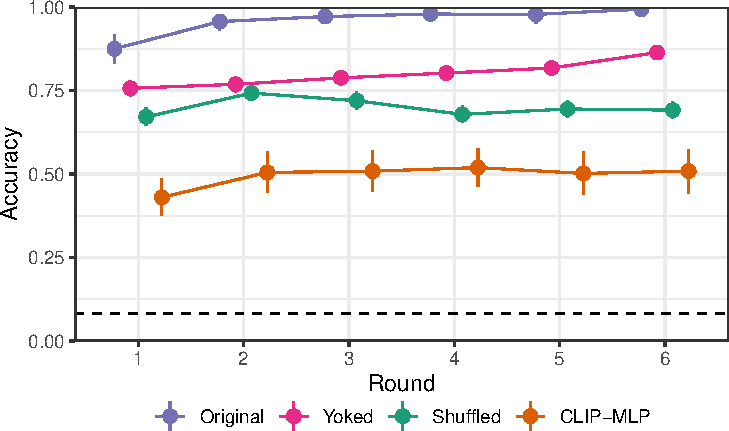
\includegraphics[width=0.9\linewidth]{figs/fig-yoked-1} 

}

\caption[Accuracies for Experiment 3]{Accuracies for Experiment 3. Error bars are bootstrapped 95\% CIs. \label{yoked}}\label{fig:fig-yoked}
\end{figure}
\end{CodeChunk}

\subsection{Results and discussion}\label{results-and-discussion-1}

Our primary question of interest was how much seeing the conversation
history unfold in order would help participants interpret descriptions,
especially those from later rounds.

We compared accuracy across the yoked and shuffled conditions with a
Bayesian mixed-effects logistic regression.\footnote{correct \({\sim}\)
  orig\_repNum \({\times}\) condition~\({+}\) matcher\_trialNum~\({+}\)
  (1\textbar gameId)~\({+}\) (1\textbar correct\_tangram)~\({+}\)
  (1\textbar workerid)}. The descriptions were more transparent when
they were presented in a yoked order (OR = 2.20 {[}1.63, 3.00{]}, Figure
\ref{yoked}). In the shuffled condition, there was no main effect of
round number (OR for one round later = 0.99 {[}0.95, 1.02{]}), but there
was a marginal interaction where the benefit of the yoked condition
decreased for later rounds (OR for one round later = 0.94 {[}0.89,
1.00{]}). This was offset by matchers in both conditions improving at
the task over time (OR for one trial later in matcher viewing order =
1.02 {[}1.02, 1.02{]}).

Comparing to the performance of in-game matchers, we separated out the
benefits of seeing the descriptions in order versus being a participant
in the group.\footnote{correct \({\sim}\) orig\_repNum \({\times}\)
  order~\({+}\) orig\_repNum \({\times}\) setting~\({+}\)
  matcher\_trialNum~\({+}\) (1\textbar gameId)~\({+}\)
  (1\textbar correct\_tangram)~\({+}\) (1\textbar workerid)} There was a
benefit to seeing the items in order (OR = 2.24 {[}1.63, 3.04{]}) and a
larger benefit to being a participant during the game (OR = 4.35
{[}2.77, 6.89{]}). The benefit of seeing the items in order waned in
later blocks (OR = 0.94 {[}0.89, 1.00{]}), but the benefit of being in
the game did not (OR = 1.06 {[}0.95, 1.18{]}). In all cases, there was a
baseline improvement over trials (OR = 1.02 {[}1.02, 1.02{]}). As a
caveat, we note that in-game matchers and naïve matchers may have varied
from each other in terms of effort and time spent on the task, and thus
the comparison should be interpreted cautiously.

The accuracy of the CLIP-MLP model was worse than the shuffled human
results, and did not change across rounds (OR for one round later = 1.02
{[}0.97, 1.07{]}). The larger difference between naïve human and
CLIP-MLP accuracies in Experiment 3 than Experiment 2 suggests that the
shuffled ordering still provides useful context that helps matchers
understand the conventions. This history was not available to the
CLIP-MLP model which saw every description as a one-shot task.

\section{General Discussion}\label{general-discussion}

Real-world conventions vary in whether they are opaque to outsiders
(``rizz'') or interpretable even to those who don't produce them
(``roundabout''). Convention formation in the real world is difficult to
study, so iterated reference games are a method for operationalizing
convention formation for experimental study. In reference games,
conventions are partner-specific: different groups' evolving conventions
follow different paths through semantic space. Despite the number of
studies on iterated reference games, few studies have examined whether
the descriptions are interpretable by outsiders.

Across multiple experiments, we found that naïve human matchers were far
above chance at identifying the targets, and our computational model was
also above chance. For both humans and models, more variation was
explained by the target image than the round or game condition the
descriptions came from, suggesting that conventionalization was not the
primary driver of how difficult an expression was to interpret. Even for
games selected for strong conventionalization, naïve matchers had high
accuracy overall, although this accuracy was further increased if they
saw the conversation history in order. Exploratory analyses also
suggested that more idiosyncratic descriptions were more opaque. Our
findings are consistent with a lexical uncertainty approach, where
expressions that are closer to overall priors are easier to understand,
and groups that have fewer people and thicker channels are more able to
break away from these priors and have conventions that drift farther
apart in semantic space.

Limiting the generality of our findings, our experimental and
computational results were only on a specific set of iterated reference
game transcripts and images. Some images may lend themselves to more
transparent descriptions because they are more iconic, with a narrower
prior over different ways they could be conceptualized, or they may be
further from competitors within this pool of images. Future work
sampling across larger sets of images (such as Ji et al., 2022) could
probe image-level factors.

Nonetheless, this work has demonstrated the utility of adopting a
broader perspective on convention comprehension. In particular, the use
of computational modelling allowed for a means to estimate semantics
under lexical uncertainty without requiring symbolic semantic
representations. Future work could capitalize on this approach to better
understand semantic dynamics underlying convention formation, as well as
provide further quantitative investigations of pragmatics models like
RSA and CHAI. These directions will help us to better understand the
nature of reference and conventions, and how humans navigate the complex
and ever-evolving landscape of communication.

\section{References}\label{references}

\setlength{\parindent}{-0.1in} 
\setlength{\leftskip}{0.125in}

\noindent

\phantomsection\label{refs}
\begin{CSLReferences}{1}{0}
\bibitem[\citeproctext]{ref-bergen2016}
Bergen, L., Levy, R., \& Goodman, N. (2016). Pragmatic reasoning through
semantic inference. \emph{Semantics and Pragmatics}, \emph{9}, 20:1--91.
\url{https://doi.org/10.3765/sp.9.20}

\bibitem[\citeproctext]{ref-bohn2022}
Bohn, M., Schmidt, L. S., Schulze, C., Frank, M. C., \& Tessler, M. H.
(2022). Modeling {Individual Differences} in {Children}'s {Information
Integration During Pragmatic Word Learning}. \emph{Open Mind}, \emph{6},
311--326. \url{https://doi.org/10.1162/opmi_a_00069}

\bibitem[\citeproctext]{ref-boyce2024}
Boyce, V., Hawkins, R., Goodman, N. D., \& Frank, M. C. (2024).
\emph{Interaction structure constrains the emergence of conventions in
group communication}.

\bibitem[\citeproctext]{ref-burkner2018}
Bürkner, P.-C. (2018). Advanced bayesian multilevel modeling with the r
package brms. \emph{The R Journal}, \emph{10}(1), 395--411.

\bibitem[\citeproctext]{ref-chen2016xgboost}
Chen, T., \& Guestrin, C. (2016). Xgboost: {A} scalable tree boosting
system. \emph{Proceedings of the 22nd Acm Sigkdd International
Conference on Knowledge Discovery and Data Mining}, 785--794.

\bibitem[\citeproctext]{ref-clark1987a}
Clark, H. H., \& Schaefer, E. F. (1987). Concealing one's meaning from
overhearers. \emph{Journal of Memory and Language}, \emph{26}(2),
209--225. \url{https://doi.org/10.1016/0749-596X(87)90124-0}

\bibitem[\citeproctext]{ref-clark1986}
Clark, H. H., \& Wilkes-Gibbs, D. (1986). \emph{Referring as a
collaborative process}.

\bibitem[\citeproctext]{ref-frank2012a}
Frank, M. C., \& Goodman, N. D. (2012). Predicting {Pragmatic Reasoning}
in {Language Games}. \emph{Science}, \emph{336}(6084), 998--998.
\url{https://doi.org/10.1126/science.1218633}

\bibitem[\citeproctext]{ref-goodman2016}
Goodman, N. D., \& Frank, M. C. (2016). Pragmatic {Language
Interpretation} as {Probabilistic Inference}. \emph{Trends in Cognitive
Sciences}, \emph{20}(11), 818--829.
\url{https://doi.org/10.1016/j.tics.2016.08.005}

\bibitem[\citeproctext]{ref-grand2022}
Grand, G., Blank, I. A., Pereira, F., \& Fedorenko, E. (2022). Semantic
projection recovers rich human knowledge of multiple object features
from word embeddings. \emph{Nature Human Behaviour}, \emph{6}(7),
975--987. \url{https://doi.org/10.1038/s41562-022-01316-8}

\bibitem[\citeproctext]{ref-gul2024}
Gul, M. O., \& Artzi, Y. (2024). \emph{{CoGen}: {Learning} from
{Feedback} with {Coupled Comprehension} and {Generation}}
(arXiv:2408.15992). arXiv.
\url{https://doi.org/10.48550/arXiv.2408.15992}

\bibitem[\citeproctext]{ref-hawkins2020b}
Hawkins, R. D., Frank, M. C., \& Goodman, N. D. (2020). Characterizing
the dynamics of learning in repeated reference games.
\emph{arXiv:1912.07199 {[}Cs{]}}. \url{https://arxiv.org/abs/1912.07199}

\bibitem[\citeproctext]{ref-hawkins2021a}
Hawkins, R. D., Franke, M., Frank, M. C., Goldberg, A. E., Smith, K.,
Griffiths, T. L., \& Goodman, N. D. (2021). \emph{From partners to
populations: {A} hierarchical {Bayesian} account of coordination and
convention} (arXiv:2104.05857). arXiv.
\url{https://doi.org/10.48550/arXiv.2104.05857}

\bibitem[\citeproctext]{ref-hawkins2021}
Hawkins, R. D., Liu, I., Goldberg, A. E., \& Griffiths, T. G. (2021).
Respect the code: {Speakers} expect novel conventions to generalize
within but not across social group boundaries. \emph{CogSci}.

\bibitem[\citeproctext]{ref-hawkins2023a}
Hawkins, R. D., Sano, M., Goodman, N. D., \& Fan, J. E. (2023). Visual
resemblance and interaction history jointly constrain pictorial meaning.
\emph{Nature Communications}, \emph{14}(1), 2199.
\url{https://doi.org/10.1038/s41467-023-37737-w}

\bibitem[\citeproctext]{ref-ji2022}
Ji, A., Kojima, N., Rush, N., Suhr, A., Vong, W. K., Hawkins, R., \&
Artzi, Y. (2022). Abstract {Visual Reasoning} with {Tangram Shapes}. In
Y. Goldberg, Z. Kozareva, \& Y. Zhang (Eds.), \emph{Proceedings of the
2022 {Conference} on {Empirical Methods} in {Natural Language
Processing}} (pp. 582--601). Association for Computational Linguistics.
\url{https://doi.org/10.18653/v1/2022.emnlp-main.38}

\bibitem[\citeproctext]{ref-kang2020}
Kang, Y., Wang, T., \& de Melo, G. (2020). Incorporating {Pragmatic
Reasoning Communication} into {Emergent Language}. \emph{Advances in
{Neural Information Processing Systems}}, \emph{33}, 10348--10359.

\bibitem[\citeproctext]{ref-le2022}
Le, H., Daryanto, T., Zhafransyah, F., Wijaya, D., Coppock, E., \& Chin,
S. (2022). \emph{Referring {Expressions} with {Rational Speech Act
Framework}: {A Probabilistic Approach}} (arXiv:2205.07795). arXiv.
\url{https://doi.org/10.48550/arXiv.2205.07795}

\bibitem[\citeproctext]{ref-leeuw2023}
Leeuw, J. R. de, Gilbert, R. A., \& Luchterhandt, B. (2023). {jsPsych}:
{Enabling} an {Open-Source Collaborative Ecosystem} of {Behavioral
Experiments}. \emph{Journal of Open Source Software}, \emph{8}(85),
5351. \url{https://doi.org/10.21105/joss.05351}

\bibitem[\citeproctext]{ref-misyak2016}
Misyak, J., Noguchi, T., \& Chater, N. (2016). Instantaneous
{Conventions}: {The Emergence} of {Flexible Communicative Signals}.
\emph{Psychological Science}, \emph{27}(12), 1550--1561.
\url{https://doi.org/10.1177/0956797616661199}

\bibitem[\citeproctext]{ref-murfitt2001}
Murfitt, T., \& McAllister, J. (2001). The {Effect} of {Production
Variables} in {Monolog} and {Dialog} on {Comprehension} by {Novel
Listeners}. \emph{Language and Speech}, \emph{44}(3), 325--350.
\url{https://doi.org/10.1177/00238309010440030201}

\bibitem[\citeproctext]{ref-muttenthaler2021}
Muttenthaler, L., \& Hebart, M. N. (2021). {THINGSvision}: {A Python
Toolbox} for {Streamlining} the {Extraction} of {Activations From Deep
Neural Networks}. \emph{Frontiers in Neuroinformatics}, \emph{15}.
\url{https://doi.org/10.3389/fninf.2021.679838}

\bibitem[\citeproctext]{ref-ohmer2022}
Ohmer, X., Franke, M., \& König, P. (2022). Mutual {Exclusivity} in
{Pragmatic Agents}. \emph{Cognitive Science}, \emph{46}(1), e13069.
\url{https://doi.org/10.1111/cogs.13069}

\bibitem[\citeproctext]{ref-pedregosa2011scikit}
Pedregosa, F., Varoquaux, G., Gramfort, A., Michel, V., Thirion, B.,
Grisel, O., Blondel, M., Prettenhofer, P., Weiss, R., Dubourg, V., et
al. (2011). Scikit-learn: {Machine} learning in python. \emph{The
Journal of Machine Learning Research}, \emph{12}, 2825--2830.

\bibitem[\citeproctext]{ref-potts2016}
Potts, C., Lassiter, D., Levy, R., \& Frank, M. C. (2016). Embedded
{Implicatures} as {Pragmatic Inferences} under {Compositional Lexical
Uncertainty}. \emph{Journal of Semantics}, \emph{33}(4), 755--802.
\url{https://doi.org/10.1093/jos/ffv012}

\bibitem[\citeproctext]{ref-radford2021}
Radford, A., Kim, J. W., Hallacy, C., Ramesh, A., Goh, G., Agarwal, S.,
Sastry, G., Askell, A., Mishkin, P., Clark, J., Krueger, G., \&
Sutskever, I. (2021). \emph{Learning {Transferable Visual Models From
Natural Language Supervision}} (arXiv:2103.00020). arXiv.
\url{https://doi.org/10.48550/arXiv.2103.00020}

\bibitem[\citeproctext]{ref-reimers2019}
Reimers, N., \& Gurevych, I. (2019). \emph{Sentence-{BERT}: {Sentence
Embeddings} using {Siamese BERT-Networks}} (arXiv:1908.10084). arXiv.
\url{https://doi.org/10.48550/arXiv.1908.10084}

\bibitem[\citeproctext]{ref-schober1989}
Schober, M. F., \& Clark, H. H. (1989). Understanding by addressees and
overhearers. \emph{Cognitive Psychology}, \emph{21}(2), 211--232.
\url{https://doi.org/10.1016/0010-0285(89)90008-X}

\bibitem[\citeproctext]{ref-schuster2020}
Schuster, S., \& Degen, J. (2020). I know what you're probably going to
say: {Listener} adaptation to variable use of uncertainty expressions.
\emph{Cognition}, \emph{203}, 104285.
\url{https://doi.org/10.1016/j.cognition.2020.104285}

\bibitem[\citeproctext]{ref-wilkes-gibbs1992}
Wilkes-Gibbs, D., \& Clark, H. (1992). Coordinating beliefs in
conversation. \emph{Journal of Memory and Language}, 183--194.

\bibitem[\citeproctext]{ref-yoon2018}
Yoon, S. O., \& Brown-Schmidt, S. (2018). Aim {Low}: {Mechanisms} of
{Audience Design} in {Multiparty Conversation}. \emph{Discourse
Processes}, \emph{55}(7), 566--592.
\url{https://doi.org/10.1080/0163853X.2017.1286225}

\end{CSLReferences}

\bibliographystyle{apacite}


\end{document}
